\section{Forecasting with machine learning}

With the webapp and database operational I moved on to attempting to forecast
the microclimate with machine learning. The idea for this model would be that I
could give it future general weather forecast data and then it would return
adjusted microclimate datapoints based on this.


\subsection{LightGBM}

LightGBM is a popular machine learning algorithm developed by Microsoft. I chose
LightGBM as it offers a good balance between performance and training efficiency
compared to similar models such as XGBoost \cite{saha2025}.

Both LightGBM and XGBoost are known as 'Gradient Boosted Machines'. This is a
relatively new technique in machine learning that effectively combines many
weaker machine learning models (called weak learners) to create a single highly
accurate model. These models are excellent for tabular data (such as my node and
forecast data) and regularly beat out competing learning algorithms
\cite{tuychiev2023}. LightGBM is also compatible with the m2cgen library that
allows the final model to be converted to javascript format, allowing it to work
within my webapp. All these factors made LightGBM a good algorthim for my use
case.

To perform the training I installed python with the lightGBM  and m2cgen
libraries as described above. I then also installed pandas for data handling
purposes.

\subsection{Machine learning process}

I aimed to create eight separate machine learning models, one for each node
(node 1 and node 2) and one for each sensor type per node (temperature,
humidity, wind speed and soil moisture). Training the model would require
"features" which are essentially the inputs to the model that it then uses to
estimate a "target" (i.e. the output).

The final models would take a 48 hour general future forecast as their input and
then output a predicted microclimate specific sensor reading (e.g. predicted
node 1 temperature). The models would be trained using historic current weather
collected from the same api and trained against actual sensor readings to create
an accurate prediction. The following diagram shows a process map this training
process:

\begin{figure}[H]
    \centering
    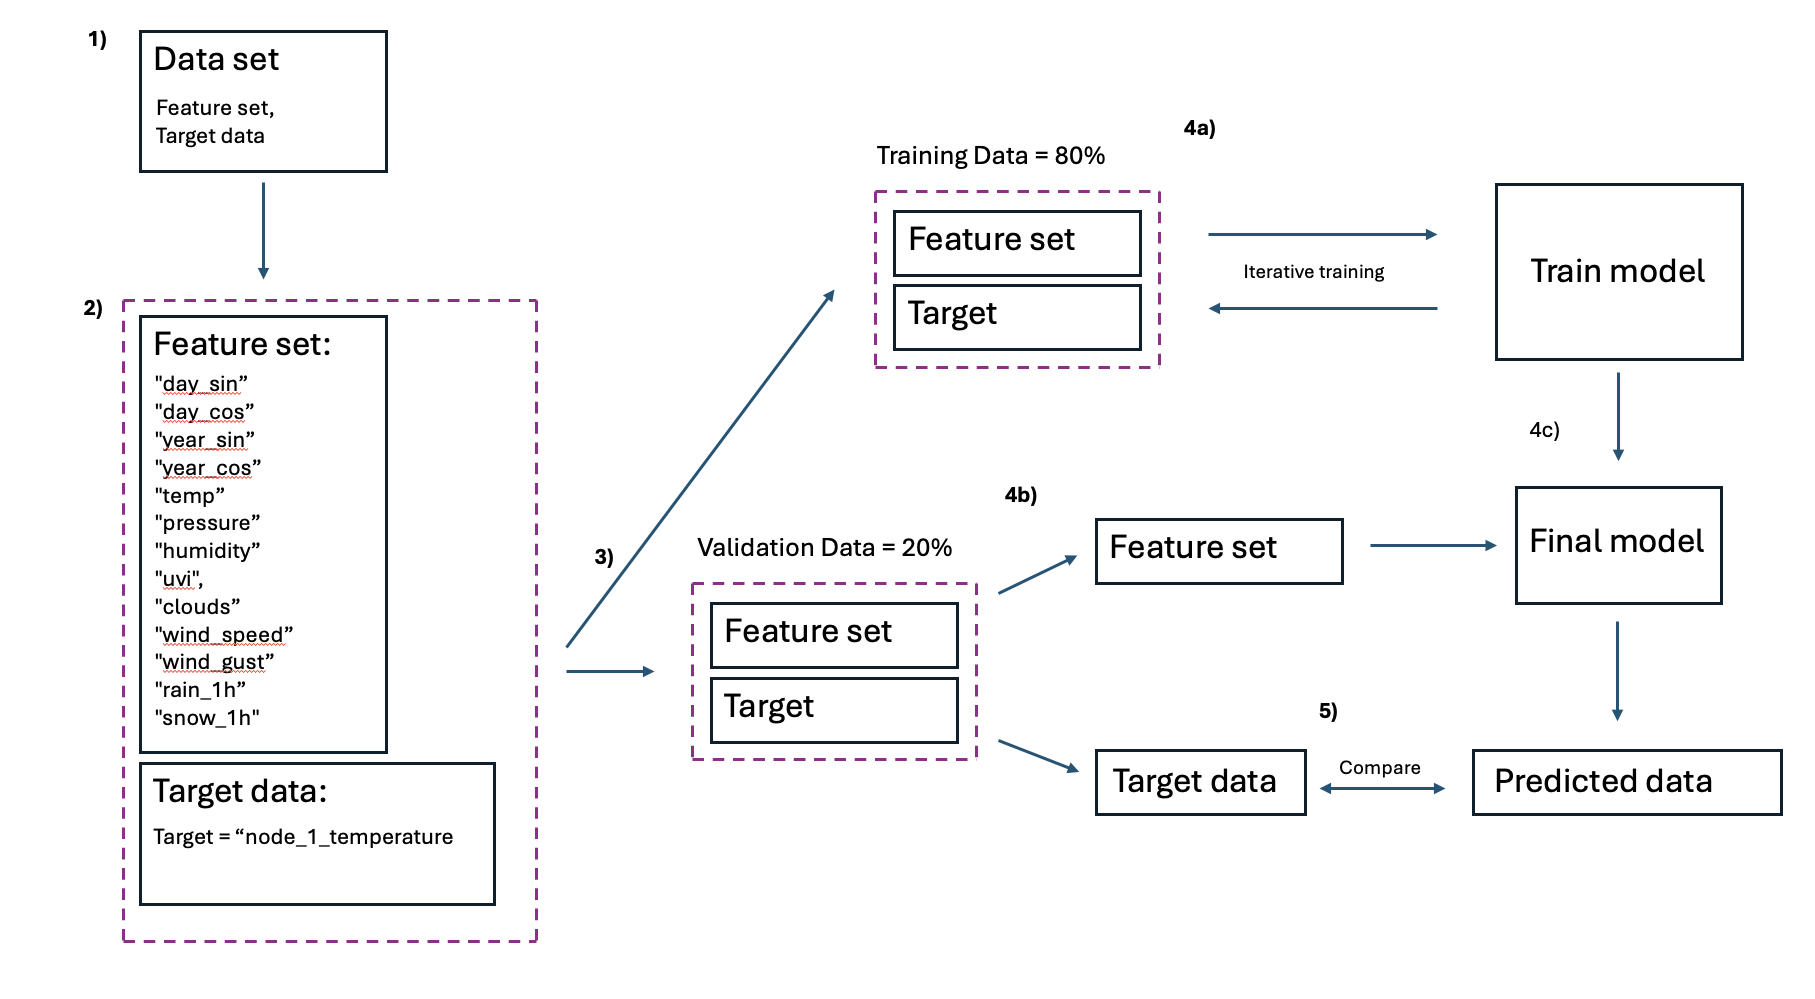
\includegraphics[width=1\textwidth]{contents/part-3/fig3/machine_learning_diagram.png}
    \caption{Infographic showing steps for training with LightGBM. This uses the temperature target for illustration.}
    \label{fig:machine_diagram}
\end{figure}

\begin{enumerate}
    \item Preparing the dataset: A single cleaned dataset was created with
    timestamps between the api weather data and node data matched. As API
    readings are taken every 10 minutes and node readings every 1 minute, 9/10
    node readings were discarded. The final dataset was roughly 1,400 rows.
    \item Define the feature set and target data:  
    The feature set (weather API) and target (node data) were defined, and
    unnecessary columns discarded. The Unix timestamp used for database purposes
    was transformed into sine and cosine representations of day and year. This
    is necessary when training a time-series data set as the algorithm must be
    able to understand the cyclical nature of time.  
    For example, using raw timestamps would incorrectly suggest to the algorithm
    that the times of 23:00 on day 1 and 00:00 on day 2 are 23 hours apart.
    \item Split the dataset into training (80\%) and validation (20\%): This
    step is necessary so that s
    \item
        \begin{enumerate}
            \item Run iterative training model: A model is trained against the
            feature set. It uses the target as supervision to get the best
            possible model.
            \item Remove target data from feature set: The validation data is
            split into feature set and target. This is so the final model can be
            tested without access to the actual data.
            \item Produce a trained model: When the model training has iterated
            at least 50 times with no improvements a final model is generated.
        \end{enumerate}
    \item Use validation feature set in final model and compare predicted data
    with actual: This step then compares how the model performs on the
    validation data compared to its performance during training. In most
    instances the model will be less accurate on validation data as it has never
    seen this before.
\end{enumerate}

With the eight models created they were then placed into the backend of the
webapp and fed new forecast data every 10 minutes to create regularly updated
predictions. The front end requests the predicted data from the backend and
displays this as a chart line.

\begin{figure}[H]
    \centering
    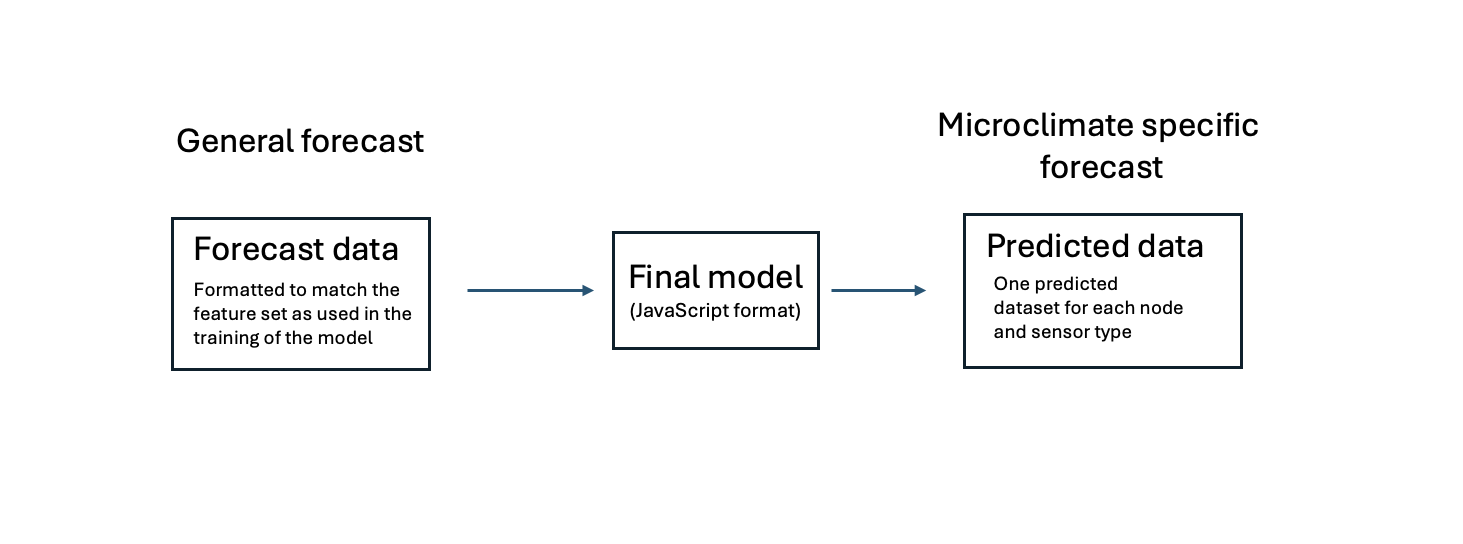
\includegraphics[width=0.8\textwidth]{contents/part-3/fig3/model_diagram.png}
    \caption{Infographic showing how final model is used on the webapp}
    \label{fig:model_diagram}
\end{figure}
